\documentclass[a4paper,12pt]{jarticle}
\usepackage[dvipdfmx]{graphicx}
\usepackage{amsmath}
\usepackage{subfigure}
\usepackage{comment}

\setlength{\hoffset}{0cm}
\setlength{\oddsidemargin}{-3mm}
\setlength{\evensidemargin}{-3cm}
\setlength{\marginparsep}{0cm}
\setlength{\marginparwidth}{0cm}
\setlength{\textheight}{24.7cm}
\setlength{\textwidth}{17cm}
\setlength{\topmargin}{-45pt}

\renewcommand{\baselinestretch}{1.6}
\renewcommand{\floatpagefraction}{1}
\renewcommand{\topfraction}{1}
\renewcommand{\bottomfraction}{1}
\renewcommand{\textfraction}{0}
\renewcommand{\labelenumi}{(\arabic{enumi})}
%\renewcommand{\figurename}{Fig.} %図をFig.にする


%図のキャプションからコロン:を消す
\makeatletter
\long\def\@makecaption#1#2{% #1=図表番号、#2=キャプション本文
\sbox\@tempboxa{#1. #2}
\ifdim \wd\@tempboxa >\hsize
#1 #2\par 
\else
\hb@xt@\hsize{\hfil\box\@tempboxa\hfil}
\fi}
\makeatother
% 


\title{電機システム制御特論 \\
Assignment (2016/05/20)\\
}
\author{\vspace{40mm}\\
九州工業大学大学院 \hspace{0mm} 工学府\\
機械知能工学専攻\ \hspace{0mm} 知能制御工学コース \\
\vspace{5mm}\\
所属:\ 西田研究室\\
学籍番号:\ 16344217\\
提出者氏名:\ 津上 \hspace{0mm} 祐典\\\vspace{5mm}\\ }
\date{平成28年\ 5月\ 27日}

\begin{document}

%表紙
\titlepage
\maketitle
\thispagestyle{empty}

\newpage

\thispagestyle{empty}
\tableofcontents

\newpage
\setcounter{page}{1}
%%%%%%%%%%%%%%%%%%%%%%%%
\section{問題}
%%%%%%%%%%%%%%%%%%%%%%%%
Consider the following system
%
\begin{eqnarray}
 \begin{cases}
  x = ax + bu + v & \\
  y = x + w
 \end{cases}
\end{eqnarray}
%

where $a=-0.02$ , $b=0.001351$, and $v$ and $w$ are both White Gaussian
noise $E \bigl\{ v^2 \bigr\} = E \bigl\{ w^2 \bigr\} = 0.7$.
Design kalman filter for the system, and demonstrate the performance
with computer simulations.

%%%%%%%%%%%%%%%%%%%%%%%%
\section{カルマンフィルタとは}
%%%%%%%%%%%%%%%%%%%%%%%%
カルマンフィルタとは,雑音が入った観測値を用いて,ある動的システムの状
態推定(フィルタリング)するものである.簡単に言うと,雑音に埋もれた信号
の中から目的の信号を取り出すフィルタである.状態方程式の状態推定する方法
として,ルーエンバーガによるオブザーバ(状態推定器)が有名であるが,これ
は雑音などが存在しない確定的な場合を対象としている.それに対して,カルマ
ンフィルタは,確定的な枠組みで状態推定問題を検討した.カルマンフィルタで
は,雑音の正規白色性を仮定することにより,システマティックに最適設計が可
能という優位点を持つ.制御対象の正確なモデルを利用できれば,状態推定
(フィルタリング)することが出来る.これは,カルマンフィルタの重要なポイ
ントである.つまり,制御対象のモデリングの正確さがカルマンフィルタの精度
に関わってくる.図\ref{fig:kalman_m}に,あるシステムにカルマンフィルタを適
応したものを示す.図\ref{fig:kalman_m}に示す一入力一出力のシステム
\begin{eqnarray}
 \begin{cases}
  \dot{x}=Ax+bu+v & \\
  y = cx + w
  \end{cases}
\end{eqnarray}
を考える.ここで$(A,c)$の組は可観測である.また,$v$はシステムノイズであ
り,$w$は観測ノイズである.これらの2つのノイズは白色ガウス雑音と
呼ばれており,システムノイズ$v(t)$,観測ノイズ$w(t)$は
\begin{equation}\label{equ:ave}
  E \bigl\{v(t)\bigr\} = 0 \ , \ E \bigl\{w(t)\bigr\} = 0 
\end{equation}
%
\begin{equation}\label{equ:soukan}
E \bigl\{v(t)v(\tau)^T\bigr\} = Q\delta (t - \tau) \ , \  E
 \bigl\{w(t)w(\tau)^T\bigr\} = r\delta (t - \tau)
\end{equation}
%
\begin{equation}\label{equ:vw}
  E \bigl\{v(t)w(\tau)\bigr\} = 0 %\ \ \ \ \ \rm{for \  all} \ t \ \rm{and} \ \tau
\end{equation}
を満たす.
%
\begin{figure}[tbp]
 \begin{center}
  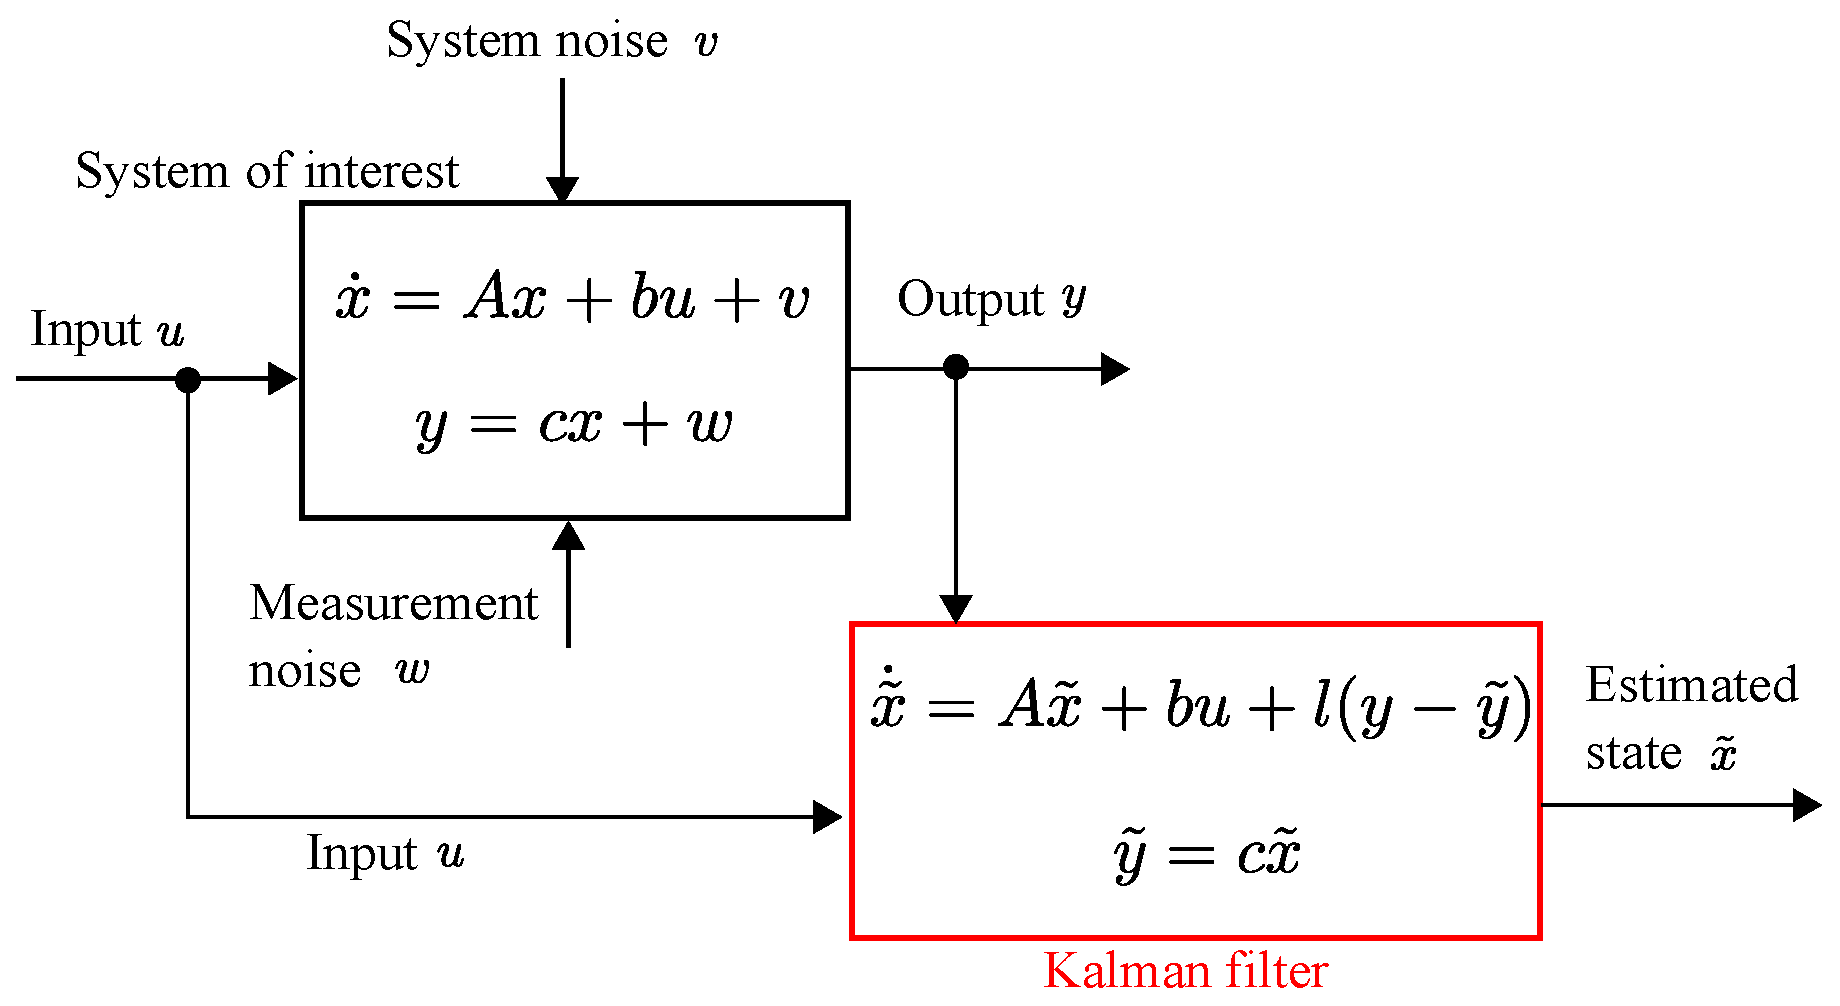
\includegraphics[width = 150mm]{fig/kalman_model.eps}
 \end{center}
 \caption{カルマンフィルタ}
 \label{fig:kalman_m}
\end{figure}
%
ここで(\ref{equ:ave})式では$v(t),w(t)$の平均が0であること,(\ref{equ:soukan})式は
$v(t)$と$w(t)$の自己相関がそれぞれ$Q,r$であ
ること,(\ref{equ:vw})式では$v(t),w(\tau)$の相互
相関が0であることを表している.

定常カルマンフィルタは同一次元オブザーバと同じ構造であり,以下の式で与え
られる.
%
\begin{eqnarray}
 \begin{cases}
\dot{\tilde{x}} = Ax + bu + l \big(y - \tilde{y} \big)
  & \\
  \tilde{y} = c\tilde{x}
 \end{cases}
\end{eqnarray}
%
同一次元オブザーバを考えるときは$l$はフィードバックゲインであり,定常カ
ルマンフィルタと考えるときはカルマンゲインである.

%%%%%%%%%%%%%%%%%%%%%%%%
\section{カルマンゲインの導出}
%%%%%%%%%%%%%%%%%%%%%%%%
この節ではカルマンゲイン$l$を導出する.前節でカルマンフィルタと同一次元
オブザーバは同じ構造であると述べた.カルマンゲイン$l$を導出することは,
同一次元オブザーバのフィードバックゲイン$l$を導出することと同じ意味であ
る.はじめに,オブザーバの推定誤差ベクトルを
\begin{equation}
 e = x - \tilde{x}
\end{equation}
とおく.すると誤差ベクトルのダイナミクスとして,
\begin{eqnarray}
 \dot{e} & = & \dot{x} - \dot{\tilde{x}} \\
 & = & (Ax+bu) - \bigl\{ A\tilde{x} + bu + l(y - \tilde{y} )\bigr\} \\
 & = & (A-lc)e
\end{eqnarray}
を得る.上式よりオブザーバの特性方程式は,
\begin{equation}\label{equ:obtk}
 {\rm{det}} (sI-A+lc)=0
\end{equation}
とわかる.ただし,$I$は単位行列である.ここで図\ref{fig:state_fb}に示すような,状態フィード
バック制御系について考える.
%
\begin{figure}[bp]
 \begin{center}
  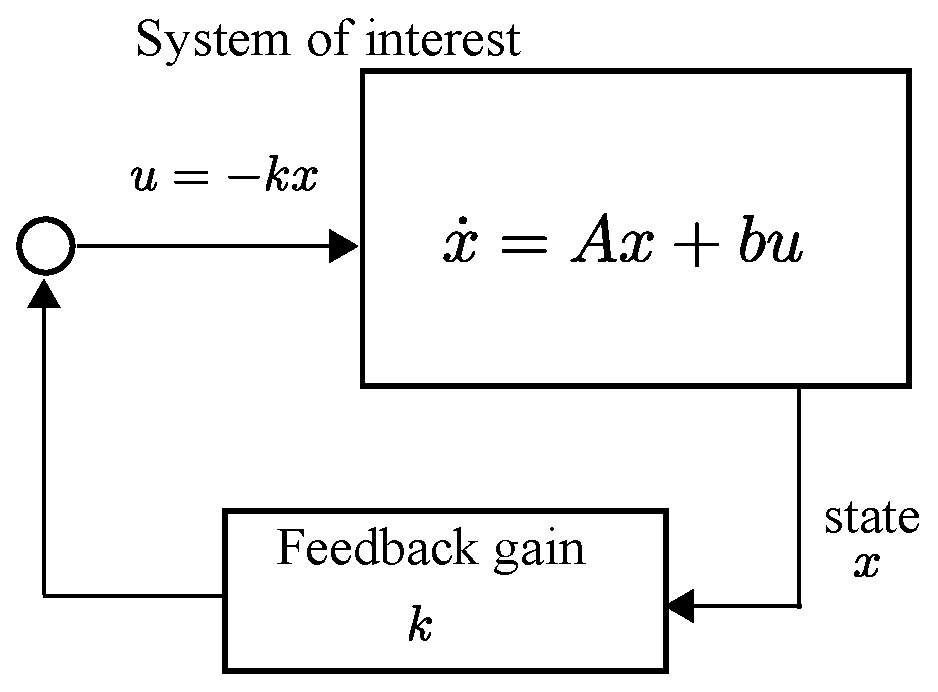
\includegraphics[width = 70mm]{fig/state_fb.eps}
 \end{center}
 \caption{状態フィードバック制御系}
 \label{fig:state_fb}
\end{figure}
%
%
\begin{figure}[tbp]
 \begin{center}
  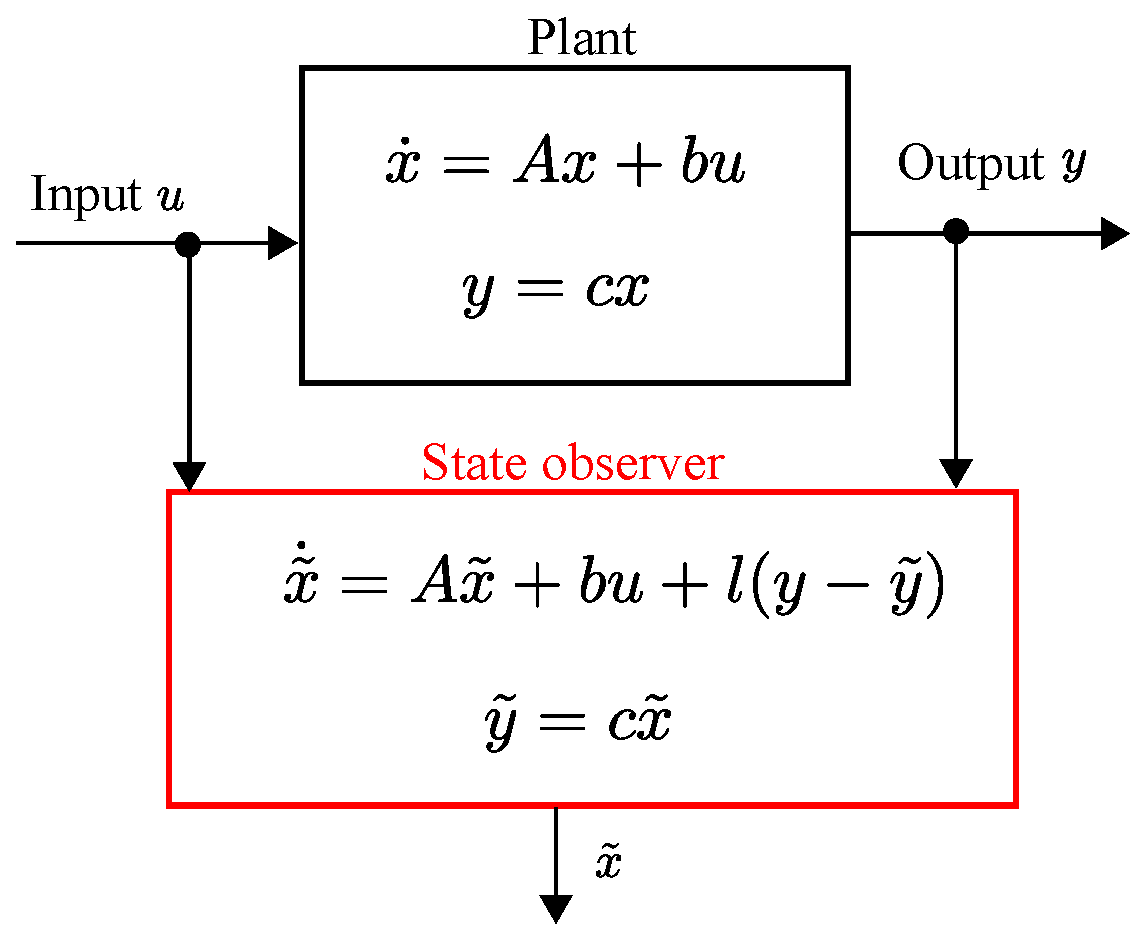
\includegraphics[width = 70mm]{fig/state_observer.eps}
 \end{center}
 \caption{状態オブザーバ}
 \label{fig:state_ob}
\end{figure}
%
このシステムの特性方程式は,
\begin{equation}\label{equ:statefb}
 {\rm{det}} (sI-A+bk)=0
\end{equation}
となる.行列$H$が正則であるとき,
\begin{equation}
 {\rm{det}} H = {\rm{det}} H^{\rm{T}}
\end{equation}
が成り立つので(\ref{equ:obtk})式は
\begin{equation}\label{equ:obtkt}
  {\rm{det}} (sI-A^{\rm{T}}+c^{\rm{T}}l^{\rm{T}})=0
\end{equation}
と書き換えることが出来る.(\ref{equ:statefb}),(\ref{equ:obtkt})式をより,
状態オブザーバ問題とレギュレータ問題に双対性があることがわかる.
オブザーバの設計に用いる係数行列$(A,b,c)$は係数行
列$(A^{\rm{T}},c^{\rm{T}},b^{\rm{T}})$で表現されるレギュレータ問題に変換
される.以下の式で表現される状態フィードバック制御系を用いてLQレギュレー
タ問題を考える.

\begin{eqnarray}\label{equ:lq}
 \begin{cases}
  \dot{x} = A^{\rm{T}}x+c^{\rm{T}}u & \\
  y = b^{\rm{T}}x & \\
  u = -l^{\rm{T}}x
 \end{cases}
\end{eqnarray}
ここで評価関数$J$を
\begin{equation}
 J  = \int_0^\infty (\dot{x}^{\rm{T}} Q x + u^{\rm{T}}ru) dt
\end{equation}
と定義する.ただし,行列$Q$は$Q \geq 0$,スカラ$r$は$r>0$を満たす.
(\ref{equ:lq})式よりリッカチ方程式は,
\begin{equation}
 AP + PA^T -\frac{1}{r}Pc^TcP = -Q 
\end{equation}
となる.これを$J$に代入する.まず,積分を抜いた式に代入すると,
\begin{eqnarray}
 \dot{x}^{\rm{T}} Q x + u^{\rm{T}} ru & = & -x^{\rm{T}}APx-x^{\rm{T}}PA^{\rm{T}}x+\frac{1}{r}x^{\rm{T}}Pcc^{\rm{T}}Px+u^{\rm{T}}ru \\
 & = & -(\dot{x}^{\rm{T}} -
  u^{\rm{T}}c)Px-x^{\rm{T}}P(\dot{x}-c^{\rm{T}}u)+\frac{1}{r}x^{\rm{T}}Pcc^{\rm{T}}Px+u^{\rm{T}}ru \\
 & = & -\dot{x}^T Px + u^T cPx -x^{\rm{T}}P\dot{x} + x^{\rm{T}}
  Pc^{\rm{T}}u + \frac{1}{r}x^{\rm{T}}Pcc^{\rm{T}}Px+u^{\rm{T}}ru \\
 & = & -2 \dot{x}^{\rm{T}}Px + u^{\rm{T}}ru + 2ru^{\rm{T}}cPx + \frac{1}{r}x^{\rm{T}}Pcc^{\rm{T}}Px
\end{eqnarray}
となる.ここで$P$は正定行列であるから,
\begin{eqnarray}
 \dot{x}^{\rm{T}} Q x + u^{\rm{T}} ru & = &  -2 \dot{x}^{\rm{T}}Px +
  r \left(u+\frac{1}{r}cPx \right)^{\rm{T}} \left(u+\frac{1}{r}cPx \right) \\
 & = & - \frac{d}{dt} \left(x^{\rm{T}} Px \right)+ r \left(u+\frac{1}{r}cPx \right)^{\rm{T}} \left(u+\frac{1}{r}cPx \right)
\end{eqnarray}
となる.レギュレータ理論において,定常状態での状態量は見かけ上$0$である.つまり$x(\infty)=0$で
あるから,評価関数$J$は,
\begin{eqnarray}
 J & = & \int_0^\infty  \Bigl\{ -\frac{d}{dt} \left(x^{\rm{T}}Px \right) +  r \left(u+\frac{1}{r}cPx \right)^{\rm{T}}
  \left(u+\frac{1}{r}cPx \right) \Bigr\} dt\\
 & = &  x^{\rm{T}}(0)Px(0)  + r \int_0^\infty \left(u+\frac{1}{r}cPx \right)^{\rm{T}}
  \left(u+\frac{1}{r}cPx \right)  dt
\end{eqnarray}
となる.すると,$J$を最小にするには制御入力$u$を
\begin{equation}
 u = - \frac{1}{r}cPx
\end{equation}
とすれば良いことがわかる.よってカルマンゲイン$l$は
\begin{equation}
 l = \frac{1}{r}Pc^T
\end{equation}
と求まる.
%%%%%%%%%%%%%%%%%%%%%%%%
\section{カルマンフィルタの設計}
%%%%%%%%%%%%%%%%%%%%%%%%
カルマンフィルタを設計するために,カルマンゲイン$l$を導出する.カルマ
ンゲインは以下の式より導出できる.
\begin{equation}\label{equ:gain}
 l = \frac{1}{r}Pc^T
\end{equation}
ただし,$P$はリッカチ方程式
\begin{equation}\label{equ:ricca}
 AP + PA^T -\frac{1}{r}Pc^TcP = -Q 
\end{equation}
の実正定行列解である.(\ref{equ:ricca})式に
\begin{eqnarray}
 \begin{cases}
  A = -0.02 & \\
  r = 0.7 & \\
  Q = 0.7 & \\
  c = 1
 \end{cases}
\end{eqnarray}
を代入し,整理すると
\begin{equation}
 P^2 + 0.028P -0.49 = 0
\end{equation}
を得る.$P > 0$より上式の解は
\begin{equation}
 P = 0.686
\end{equation}
となる.するとカルマンゲイン$l$は,
\begin{equation}
 l = \frac{1}{0.7} \times 0.686 \times 1 = 0.98
\end{equation}
となる.したがってカルマンフィルタは以下の式で与えられる.
\begin{eqnarray}
 \begin{cases}
\dot{\tilde{x}} = -0.02x + 0.001351u + 0.98 \big(y - \tilde{y} \big)
  & \\
  \tilde{y} = \tilde{x}
 \end{cases}
\end{eqnarray}


%%%%%%%%%%%%%%%%%%%%%%%%
\section{シミュレーション}
%%%%%%%%%%%%%%%%%%%%%%%%
制御入力(ステップ入力)$u$を$u=1000$としてMATLAB/Simulinkでシミュレーションを行った.こ
のとき,構成したSimulinkのモデルを図\ref{fig:kalman_b}に示す.また,シミュ
レーション結果を図\ref{fig:kalman_g}に示す.また,図\ref{fig:kalman_g}の
拡大図を図\ref{fig:kalman_B}に示す.ただし,システムノイズ$v$を
$v=0$とし,シミュレーションを行った.
%
\begin{figure}[tbp]
 \begin{center}
  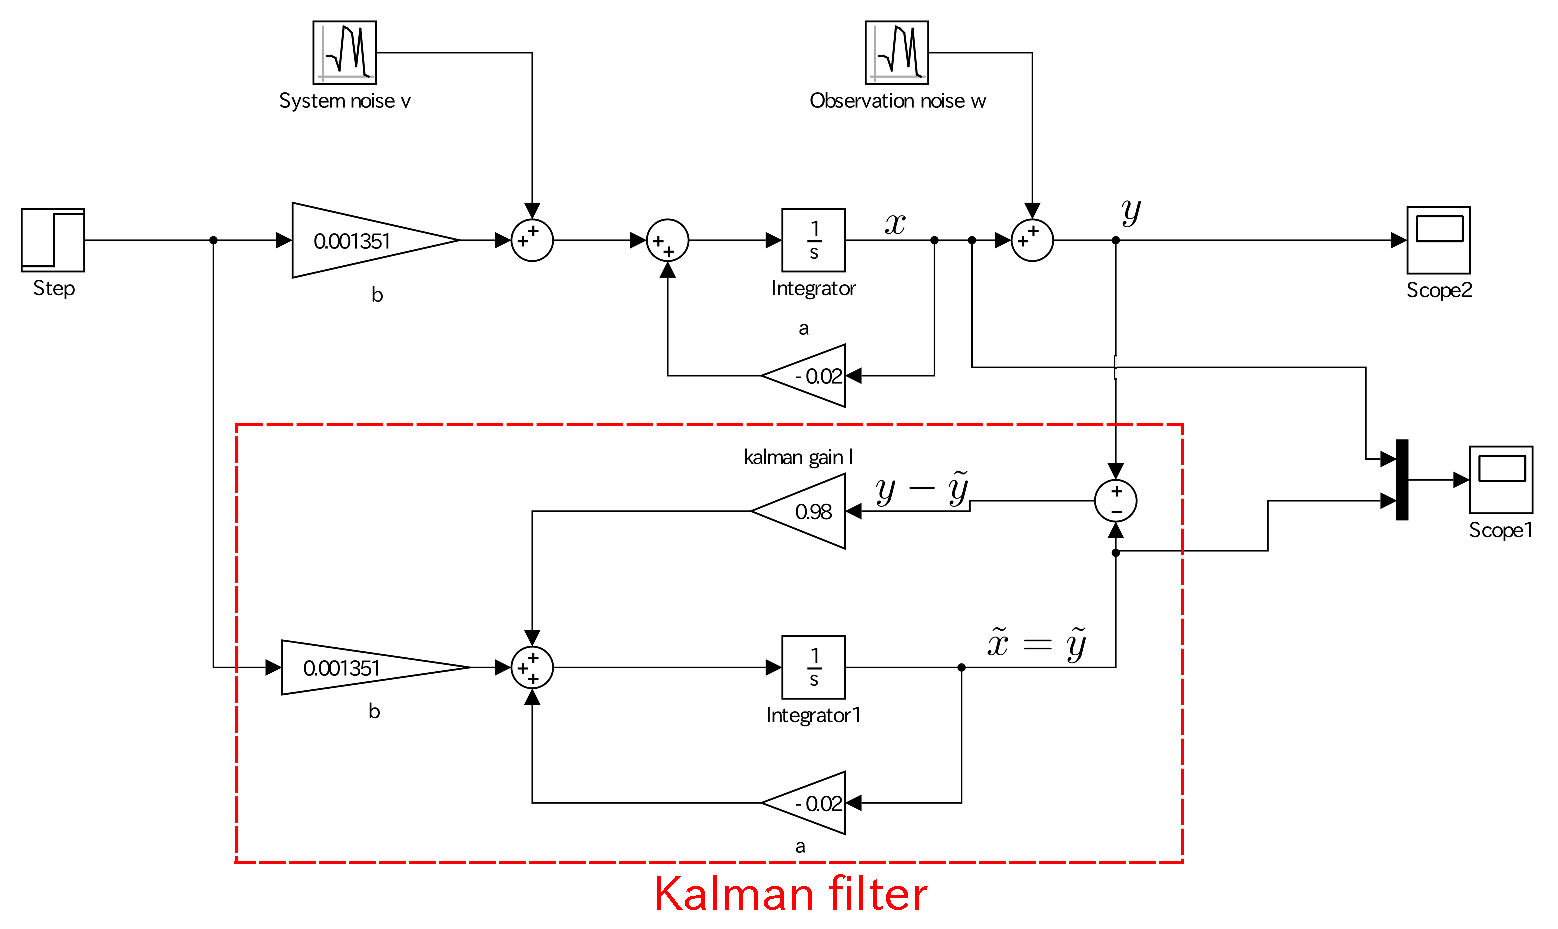
\includegraphics[width = 150mm]{fig/kalmanfilter2.eps}
 \end{center}
 \caption{simulinkで構成したモデル}
 \label{fig:kalman_b}
\end{figure}
%
\begin{figure}[htbp]
 \begin{center}
  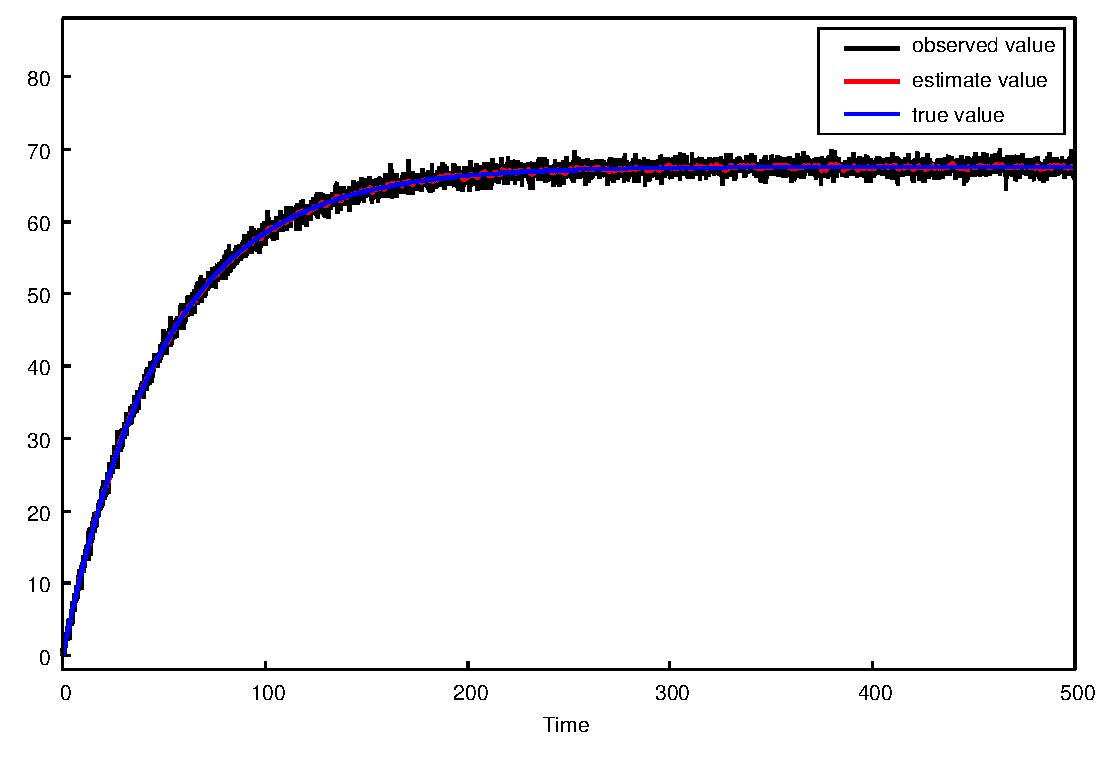
\includegraphics[width = 150mm]{fig/kalmanfilterG.eps}
 \end{center}
 \caption{シミュレーション結果}
 \label{fig:kalman_g}
\end{figure}
%
\begin{figure}[htbp]
 \begin{center}
  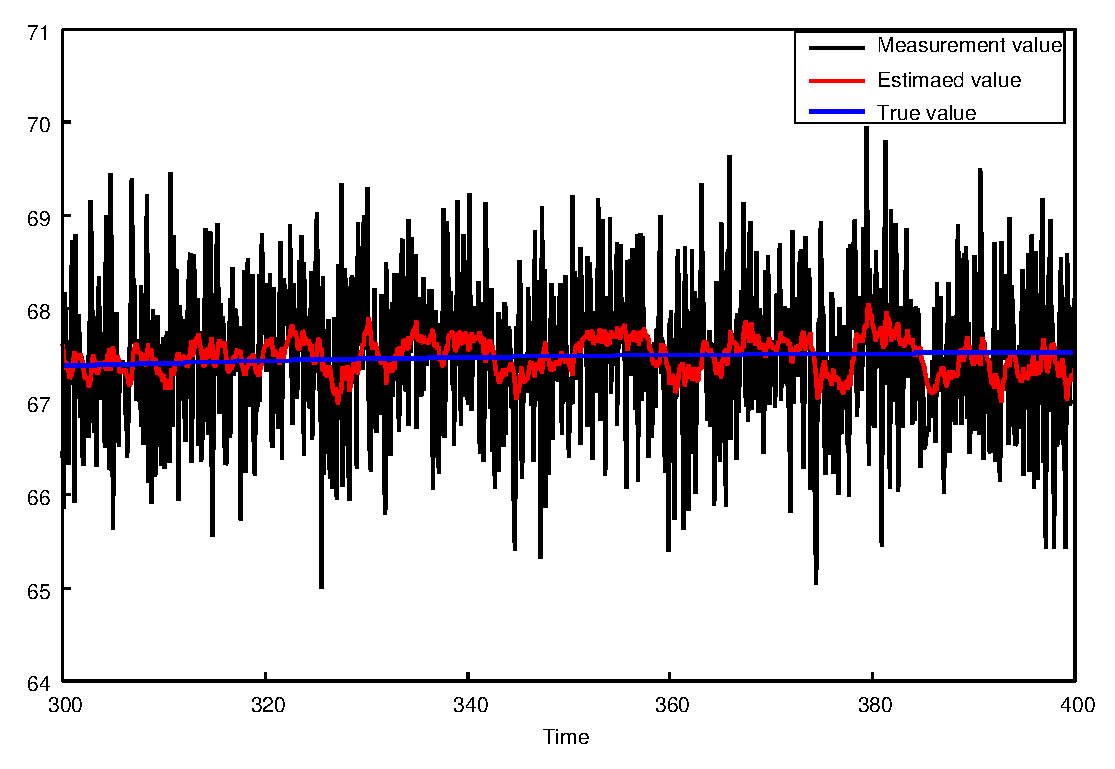
\includegraphics[width = 150mm]{fig/kalmanfilterB.eps}
 \end{center}
 \caption{シミュレーション結果(Timeが300から400のとき)}
 \label{fig:kalman_B}
\end{figure}
%
\newpage
%
%%%%%%%%%%%%%%%%%%%%%%%%
\section{考察}
%%%%%%%%%%%%%%%%%%%%%%%%
図\ref{fig:kalman_g},\ref{fig:kalman_B}を見ると,カルマンフィ
ルタを用いた推定値($\tilde{y}=\tilde{x}$)が測定値($y=x+w$)より観測ノ
イズを除いた真値($y=x$)との誤差が小さいことがわかる.つまり,カルマンフィ
ルタを使ったことにより観測ノイズの影響を抑えていることがわかる.
%
本レポートでは,システムノイズや観測ノイズの分散が既知としてシミュレーションを行っ
たが,現実世界ではノイズの正確な分散を得るのは難しい.よって,カルマンゲ
イン$l$を時間ごとに更新する必要があると考えられる.これを実現するには定
常カルマンゲインでなく,時変カルマンフィルタにしなければならない.時変カ
ルマンフィルタは以下の式で与えられる.
\begin{eqnarray}
 \begin{cases}
  \dot{\tilde{x}}=A(t) \tilde{x} + B(t)u + l(t)(\tilde{y} - y) & \\
  y = C(t)\tilde{x}
 \end{cases}
\end{eqnarray}
また,カルマンゲイン$l(t)$は
\begin{equation}
 l(t) = - \frac{1}{r}P(t)C^{\rm{T}}(t)
\end{equation}
で与えられる.ただし,共分散行列の推定値$P(t)$は$P(t)$に関するリッカチ微
分方程式
\begin{equation}
 \dot{P}(t) = A(t)P(t)+P(t)A^{\rm{T}}(t)+Q(t)-\frac{1}{r}P(t)C^{\rm{T}(t)}C(t)P(t)
\end{equation}
の解である.ただし,$\tilde{x}(0)=E \bigl\{ x(0)
\bigr\},P(0)=E\bigl\{(x(0) - E \bigl\{ x(0) \bigr\})^{\rm{T}}(x(0) - E
\bigl\{ x(0)\bigr\})\bigr\}$である.
また,2節で述べたように制御対象のモデル化の精度に
状態推定の精度が関わってくる.現実世界のプラントにカルマンフィルタを適応
する場合は,プラントをモデル化する際,低次元で近似しないように気をつける
必要があると考えられる.
%
%%%%%%%%%%%%%%%%%%%%%%%%
\section{まとめ}
%%%%%%%%%%%%%%%%%%%%%%%%
カルマンフィルタについて説明し,最適レギュレータ
問題を解くことでカルマンゲイン$l$を導出した.また,シミュレーションを行
い,考察した.
%
\begin{thebibliography}{99}
\addcontentsline{toc}{section}{参考文献}

 \bibitem{denki} T.Sakamoto,
		 "Lecture Notes of Advanced Electrical Drive Control System",
		 2016.

 \bibitem{adachi} 足立修一,丸田一郎,"カルマンフィルタの基礎",東京電機
		 大学出版局,2014.

 \bibitem{hori} 堀洋一,大西公平,"応用制御工学",丸善株式会社,1998.

 \bibitem{kanai} 金井喜美雄,"適応制御入門",オーム社,1986.

 \bibitem{mecha} 坂本哲三,"電気機器の電気力学と制御", 森北出版, 2007.

 \bibitem{digital} 山下裕,"ディジタル制御",http://stlab.ssi.ist.hokudai.ac.jp/yuhyama/lecture/digital/digi-part2.pdf.
		 
\end{thebibliography}

\end{document}
